% !TEX program = xelatex
% Clean CV template — Letter (8.5×11in) — requires XeLaTeX
% -------------------------------------------------------------
\documentclass[10pt,letterpaper]{article}

% ---------- FONTS ---------------------------------------------
\usepackage{fontspec}
\IfFontExistsTF{Roboto}
    {\setmainfont{Roboto}}
    {\IfFontExistsTF{Helvetica Neue}
        {\setmainfont{Helvetica Neue}}
        {\setmainfont{Latin Modern Sans}}}

% ---------- GEOMETRY ------------------------------------------
\usepackage[
  letterpaper,
  left=0.55in, right=0.55in,
  top=0.8in,  bottom=0.8in
]{geometry}

% ---------- COLOURS & GRAPHICS --------------------------------
\usepackage[dvipsnames,svgnames,x11names]{xcolor}
\definecolor{primary}{HTML}{004A99}
\definecolor{accent}{HTML}{E6F4FF}

\usepackage{graphicx}
\usepackage{tikz}
\usetikzlibrary{calc}

% ---------- LAYOUT HELPERS ------------------------------------
\usepackage{paracol}
\columnratio{0.32}
\setlength{\columnsep}{0.25in}

\usepackage[most]{tcolorbox}
\tcbset{colback=accent, colframe=accent, boxrule=0pt, sharp corners}

\usepackage{enumitem}
\setlist[itemize]{noitemsep,topsep=0pt,leftmargin=*}

\usepackage{sectsty}
\allsectionsfont{\color{primary}\bfseries\uppercase}
\subsectionfont{\color{primary}\bfseries}
\renewcommand{\thesection}{}

% ---------- PLACEHOLDER MACRO ---------------------------------
\newcommand{\tpl}[1]{\textcolor{Gray}{\texttt{\{\{#1\}\}}}}

% ---------- UTILITIES -----------------------------------------
\newcommand{\cvName}[1]{\vspace*{0.3in}\textbf{\LARGE #1}}
\newcommand{\cvHeadline}[1]{\par\smallskip\textit{#1}}
\newcommand{\cvHr}{\vspace{0.5\baselineskip}\hrule height 1pt\color{primary}\vspace{0.7\baselineskip}}

% ==============================================================
\begin{document}\small
\begin{paracol}{2}

% ================== SIDEBAR ====================================
\begin{leftcolumn}
\begin{center}
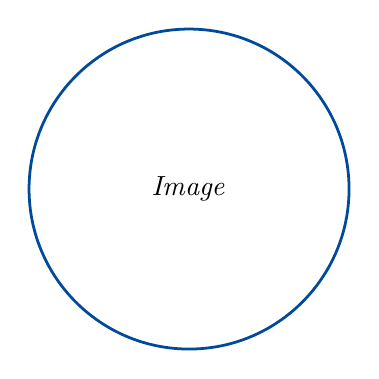
\begin{tikzpicture}
  \node[draw=primary,line width=1pt,circle,minimum width=1.6in]  {\textit{Image}};
\end{tikzpicture}
\end{center}

\vspace{0.6in}

\cvName{\tpl{name}}
\cvHeadline{\tpl{headline}}
\cvHr

\section*{Contact}
\tpl{phone}\\
\tpl{email}\\
\tpl{linkedin}\\
\tpl{address}\\
\tpl{website}

\cvHr
\section*{Languages}
\tpl{languages[0].name}\\
\tpl{languages[1].name}

\cvHr
\section*{Key Skills}
\tpl{skills[0]}\\
\tpl{skills[1]}\\
\tpl{skills[2]}\\
\tpl{skills[3]}
\end{leftcolumn}

% ================== MAIN COLUMN ================================
\begin{rightcolumn}
\section*{Professional Summary}
\tpl{summary}

\vspace{1in}
\section*{Work Experience}

\begin{tcolorbox}
  \begin{minipage}[t]{0.48\linewidth}
    \tpl{experiences[0].start}\\
    \textbf{\tpl{company[0]}}\\
    \begin{itemize}
      \item \tpl{experiences[0].description}
    \end{itemize}
  \end{minipage}\hfill
  \begin{minipage}[t]{0.48\linewidth}\raggedleft
    \tpl{experiences[0].end}
  \end{minipage}
\end{tcolorbox}

\vspace{0.9in}
\section*{Education}
\begin{tcolorbox}[colback=white,boxrule=1pt,colframe=primary]
  \tpl{degree[0].title}\\
  \tpl{degree[0].school}\\
  \tpl{degree[0].subject}\\
  \tpl{degree[0].year}
\end{tcolorbox}

\section*{Certifications}
\begin{itemize}
  \item \tpl{certification[0]}
  \item \tpl{certification[1]}
\end{itemize}

\end{rightcolumn}
\end{paracol}
\end{document}
